
In  Chapter \ref{chapter:DDP} we considered multi-stage decision
problems for \emph{deterministic} systems. In many problems of
interest, the system dynamics also involves \emph{randomness}, which
leads us to stochastic decision problems. In this chapter we
introduce the basic model of Markov Decision Processes (MDP), which
will be considered in the rest of the book, and discuss the finite
horizon return.



\section{Controlled Markov Chains}

A Markov Decision Process consists of two main parts:
\begin{enumerate}
  \item A controlled dynamic system, with stochastic evolution.
  \item A performance objective to be optimized.
\end{enumerate}
In this section we describe the first part, which is modeled as a controlled Markov chain.

Consider a controlled dynamic system, defined over:
\begin{itemize}
  \item A discrete time axis ${\mathbb{T}} = \{ 0,1, \ldots ,\tHorizon - 1\} $  (finite horizon), or
  ${\mathbb{T}} = \{ 0,1,2, \ldots \} $ (infinite horizon).
To simplify the discussion we refer below to the infinite horizon
case, which can always be ``truncated" at $\tHorizon$ if needed.
  \item A finite state space $\States$, where ${\States_\ttime} \subset \States$ is the set of possible states at time $\ttime\in {\mathbb{T}}$.
  \item A finite action set $\Actions$, where ${\Actions_\ttime}(\state) \subset \Actions$ is the set of possible actions at time $\ttime\in {\mathbb{T}}$ and state $\state \in {\States_\ttime}$.
\end{itemize}

\paragraph{State transition probabilities:}
\begin{itemize}
\item   Suppose that at time $\ttime$ we are in state ${\state_\ttime} = \state$, and choose an action ${\action_\ttime} = \action$. The next state ${\state_{\ttime + 1}} = \state'$ is then determined randomly according to a probability distribution  ${p_\ttime}( \cdot |\state,\action)$ on ${\States_{\ttime + 1}}$. That is,
\[\Pr({\state_{\ttime + 1}} = \state'|{\state_\ttime} = \state,{\action_\ttime} = \action) = {p_\ttime}(\state'|\state,\action),\quad      \quad \state' \in {\States_{\ttime + 1}}\]
\item   The probability ${p_\ttime}(\state'|\state,\action)$ is the \emph{transition probability} from state $\state$ to state $\state'$ for a given action $\action$. We naturally require that
            ${p_\ttime}(\state'|\state,\action) \ge 0$, and $\sum\nolimits_{\state' \in {\States_{\ttime + 1}}}^{} {{p_\ttime}(\state'|\state,\action)}  = 1$ for all $\state \in {\States_\ttime},\action \in {\Actions_\ttime}(\state)$.
\item   Implicit in this definition is the controlled-Markov property:
\[
\Pr({\state_{\ttime + 1}} =
\state'|{\state_\ttime},{\action_\ttime}, \ldots
,{\state_{0,}}{\action_0}) =\Pr({\state_{\ttime + 1}} =
\state'|{\state_\ttime},{\action_\ttime})
\]
\item   The set of probability distributions
                                \[P = \{ {p_\ttime}( \cdot |\state,\action)\;\;:\;\;\state \in {\States_\ttime},\action \in {\Actions_\ttime}(\state),\ttime \in {\T}\} \]
is called the \emph{transition law} or \emph{transition kernel} of the controlled Markov process.
\end{itemize}

\paragraph{Stationary Models:}
    The controlled Markov chain is called stationary or time-invariant if the transition probabilities do not depend on the time $\ttime$. That is:
                     \[\forall t,\quad {p_\ttime}(\state'|\state,\action) \equiv p(\state'|\state,\action),\;\;{\States_\ttime} \equiv \States,\;\;{\Actions_\ttime}(\state) \equiv \Actions(\state).\]

\paragraph{Graphical Notation:}
The state transition probabilities of a Markov chain are often illustrated via a state transition diagram, such as in Figure \ref{fig:MC}.

\begin{figure}
  % Requires \usepackage{graphicx}
  \begin{centering}
  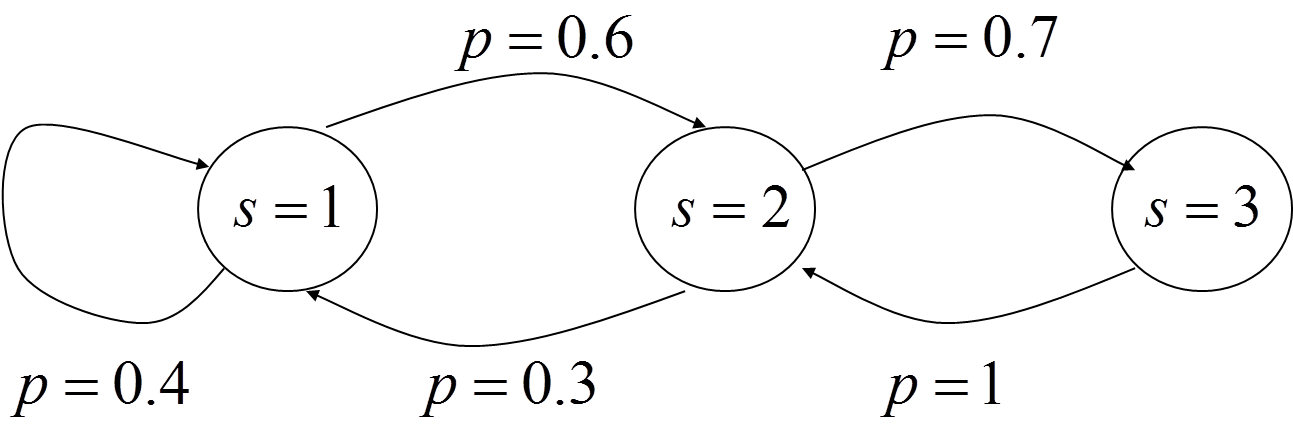
\includegraphics[width=0.7\textwidth]{figures/lecture4_a}\\
  \caption{Markov chain}\label{fig:MC}
  \end{centering}
\end{figure}

A graphical description of a controlled Markov chain is a bit more
complicated because of the additional action variable. We obtain the
diagram (drawn for state $\state = 1$ only, and for a given time
$\ttime$) in Figure \ref{fig:MDP}, reflecting the following
transition probabilities:
\[\begin{array}{l}
p(\state' = 2|\state = 1,\action = 1) = 1\\
p(\state'|\state = 1,\action = 2) = \left\{ {\begin{array}{*{20}{c}}
{0.3}&:&{\state' = 1}\\
{0.2}&:&{\state' = 2}\\
{0.5}&:&{\state' = 3}
\end{array}} \right.
\end{array}\]

\begin{figure}
  % Requires \usepackage{graphicx}
  \begin{centering}
  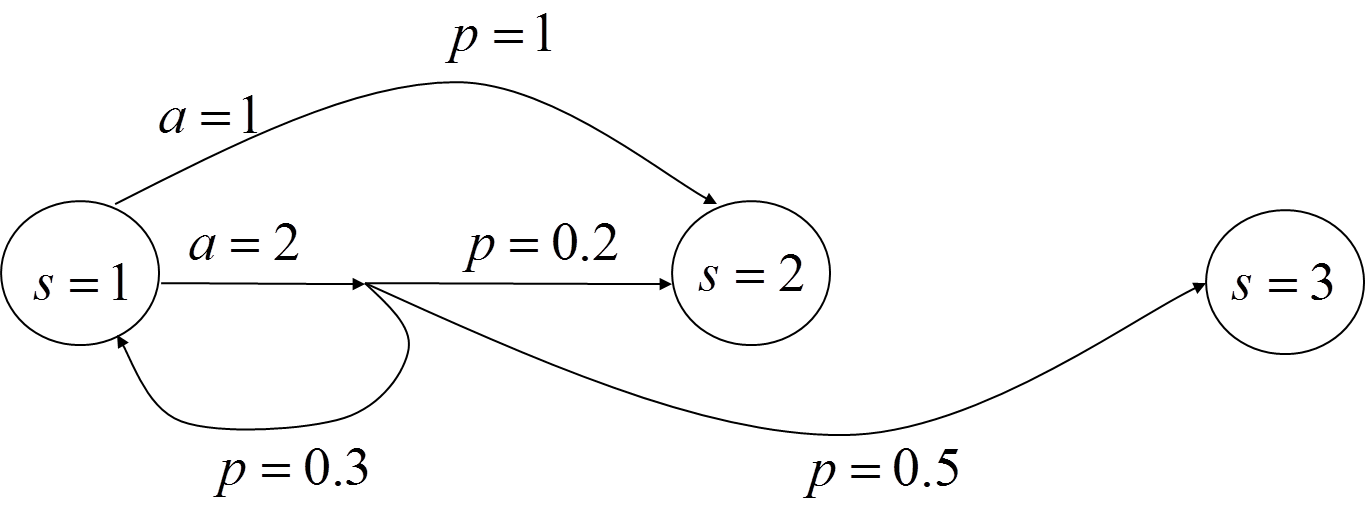
\includegraphics[width=0.7\textwidth]{figures/lecture4_b}\\
  \caption{Controlled Markov chain}\label{fig:MDP}
  \end{centering}
\end{figure}


\paragraph{State-equation notation:}
The stochastic state dynamics can be equivalently defined in terms of a state equation of the form
                                                   \[{\state_{\ttime + 1}} = {f_\ttime}({\state_\ttime},{\action_\ttime},{w_\ttime}),\]
where ${w_\ttime}$ is a random variable (RV).
    If  ${({w_\ttime})_{t \ge 0}}$ is a sequence of independent RVs, and further each ${w_\ttime}$ is independent of the ``past"  $({\state_{\ttime - 1}},{\action_{\ttime - 1}}, \ldots {\state_0})$, then ${({\state_\ttime},{\action_\ttime})_{t \ge 0}}$ is a controlled Markov process.
    For example, the state transition law of the last example can be written in this way, using
                  ${w_\ttime} \in \{ 4,5,6\} $,  with  ${p_w}(4) = 0.3,\;{p_w}(5) = 0.2,\;{p_w}(6) = 0.5$
and, for ${\state_\ttime} = 1$:
    \[\begin{array}{l}
    {f_\ttime}(1,1,{w_\ttime}) = 2\\
    {f_\ttime}(1,2,{w_\ttime}) = {w_\ttime} - 3
    \end{array}\]
  This state algebraic equation notation is especially useful for problems with continuous state space, but also for some models with discrete states.
Equivalently, we can write
    \[
 {f_\ttime}(1,2,{w_\ttime}) = 1\cdot \I[{w_\ttime}=4]+2\cdot \I[{w_\ttime}=5]+3\cdot \I[{w_\ttime}=6] ,
    \]
where $\I[\cdot]$ is the indicator function.

Next we recall the definitions of control policies from Chapter \ref{chapter:DDP}.

\paragraph{Control Policies}
\begin{itemize}
  \item
A general or \textbf{history-dependent deterministic} control policy
$\policy  = {({\policy _\ttime})_{\ttime \in {\mathbb{T}}}}$ is a
mapping from each possible history ${\history_\ttime} =
({\state_0},{\action_0}, \ldots ,{\state_{\ttime -
1}},{\action_{\ttime - 1}},{\state_\ttime})$, and time $\ttime \in
\T$, to an action ${\action_\ttime} = {\policy
_\ttime}({\history_\ttime}) \in {\Actions_\ttime}$.  We denote the
set of general policies by ${\Pi _{HD}}$.
  \item
A \textbf{Markov deterministic} control policy $\policy $ is allowed
to depend on the current state and time only: ${\action_\ttime} =
{\policy _\ttime}({\state_\ttime})$.   We denote the set of Markov
deterministic policies by ${\Pi _{MD}}$.
  \item
For stationary models, we may define \textbf{stationary
deterministic} control policies that depend on the current state
alone. A stationary policy is defined by a single mapping $\policy
:\States \to \Actions$, so that  ${\action_\ttime} = \policy
({\state_\ttime})$ for all $\ttime \in {\T}$. We denote the set of
stationary policies by ${\Pi _{SD}}$.
  \item Evidently, ${\Pi_{HD}} \supset {\Pi_{MD}} \supset {\Pi_{SD}}$.
\end{itemize}

\paragraph{Randomized Control policies}
\begin{itemize}
  \item The control policies defined above specify deterministically the action to be taken at each stage. In some cases we want to allow for a random choice of action.
  \item A general randomized control policy assigns to each possible history ${\history_\ttime}$ a probability distribution ${\policy _\ttime}( \cdot |{\history_\ttime})$ over the action set ${\Actions_\ttime}$.
  That is,  $\Pr( {\action_\ttime} = \action|{\history_\ttime})  = {\policy _\ttime}(\action|{\history_\ttime})$. We denote the set of history-dependent stochastic policies by ${\Pi _{HS}}$.
  \item Similarly, we can define the set ${\Pi _{MS}}$ of Markov stochastic control policies, where ${\policy _\ttime}( \cdot |{\history_\ttime})$ is replaced by ${\policy _\ttime}( \cdot |{\state_\ttime})$, and the set ${\Pi _{SS}}$ of stationary stochastic control policies, where ${\policy _\ttime}( \cdot |{\state_\ttime})$ is replaced by  $\policy ( \cdot
  |{\state_\ttime})$, namely the policy is independent of the time.
  \item Note that the set ${\Pi _{HS}}$ includes all other policy sets as special cases.
\end{itemize}

\paragraph{The Induced Stochastic Process}
Let  ${p_0} = \{ {p_0}(\state),\state \in {\States_0}\} $ be a
probability distribution for the initial state ${\state_0}$. (Many
time we will assume that the initial state is deterministic and
given by $\state_0$.) A control policy $\policy \in {\Pi _{HS}}$,
together with the transition law $P = \{
{p_\ttime}(\state'|\state,\action)\} $ and the initial state
distribution ${p_0} = ({p_0}(\state),\;\state \in {\States_0})$,
induces a probability distribution over any finite state-action
sequence ${\history_\tHorizon} = ({\state_0},{\action_0}, \ldots
,{\state_{\tHorizon - 1}},{\action_{\tHorizon -
1}},{\state_\tHorizon})$, given by
\[\Pr({\history_\tHorizon}) = {p_0}({\state_0})\prod\limits_{t = 0}^{\tHorizon -1} {p_\ttime({\state_{\ttime + 1}}|{\state_\ttime},{\action_\ttime}){\policy _\ttime}({\action_\ttime}|{\history_\ttime})} ,\]
where ${\history_\ttime} = ({\state_0},{\action_0}, \ldots
,{\state_{\tHorizon -1}},{\action_{\tHorizon -1}},{\state_\ttime})$.
%
To see this, observe the recursive relation:
%\[
\begin{align*}
\Pr({\history_{\ttime + 1}}) &= \Pr({\history_\ttime},{\action_\ttime},{\state_{\ttime + 1}}) = \Pr({\state_{\ttime + 1}}|{\history_\ttime},{\action_\ttime})\Pr({\action_\ttime}|{\history_\ttime})\Pr({\history_\ttime})\\
 &= {p_\ttime}({\state_{\ttime + 1}}|{\state_\ttime},{\action_\ttime}){\policy _\ttime}({\action_\ttime}|{\history_\ttime})\Pr({\history_\ttime}).
\end{align*}
%\]
In the last step we used the conditional Markov property of the
controlled chain: $\Pr({\state_{\ttime +
1}}|{\history_\ttime},{\action_\ttime}) = {p_\ttime}({\state_{\ttime
+ 1}}|{\state_\ttime},{\action_\ttime})$, and the definition of the
control policy $\policy_\ttime $. The required formula follows by
recursion.

Therefore, the state-action sequence ${\history_\infty } =
{({\state_k},{\action_k})_{k \ge 0}}$ can now be considered a
stochastic process. We denote the probability law of this stochastic
process by ${\Pr^{\policy ,{p_0}}}( \cdot )$. The corresponding
expectation operator is denoted by ${\E^{\policy ,{p_0}}}( \cdot )$.
When the initial state ${\state_0}$ is deterministic (i.e.,
${p_0}(\state)$ is concentrated on a single state $\state$), we may
simply write ${\Pr^{\policy ,s}}( \cdot )$  or ${\Pr^\policy }( \cdot
|{\state_0} = \state)$.

Under a Markov control policy, the state sequence
${({\state_\ttime})_{\ttime \ge 0}}$ becomes a \emph{Markov chain},
with transition probabilities:
\[\Pr({\state_{\ttime + 1}} = \state'|{\state_\ttime} = \state) = \sum\nolimits_{\action \in {\Actions_\ttime}} {{p_\ttime}} (\state'|\state,\action){\policy _\ttime}(\action|\state).\]
This follows since:
\begin{align*}
\Pr({\state_{\ttime + 1}} = \state'|{\state_\ttime} = \state) & =
\sum\nolimits_{\action \in {\Actions_\ttime}} \Pr({\state_{\ttime +
1}} = \state', \action|{\state_\ttime} = \state)  \\
& =\sum\nolimits_{\action \in {\Actions_\ttime}} \Pr({\state_{\ttime
+ 1}} = \state'|{\state_\ttime} = \state,\action) \Pr(\action |
\state_\ttime=\state) \\
&= \sum\nolimits_{\action \in {\Actions_\ttime}} {{p_\ttime}}
(\state'|\state,\action){\policy _\ttime}(\action|\state)
\end{align*}
 \ymignore{
\begin{exercise}{Prove this!}\end{exercise}
}

%\begin{proof} add \end{proof}

If the controlled Markov chain is stationary (time-invariant) and the control policy is stationary, then the induced Markov chain is stationary as well.



\begin{remark}
For most non-learning optimization problems, Markov policies suffice to achieve the optimum.
\end{remark}
\begin{remark}
Implicit in these definitions of control policies is the assumption
that the current state ${\state_\ttime}$ can be fully observed
before the action ${\action_\ttime}$ is chosen . If this is not the
case we need to consider the problem of a Partially Observed MDP
(POMDP), which is more involved and will be discussed in Chapter \ref{chapter:POMDP}.
\end{remark}

\section{Performance Criteria}

\subsection{Finite Horizon Return}
Consider the finite-horizon return, with a fixed time horizon
$\tHorizon$. As in the deterministic case, we are given a running
reward function ${\reward_\ttime} = \{
{\reward_\ttime}(\state,\action):\state \in {\States_\ttime},\action
\in {\Actions_\ttime}\} $ for $0 \le \ttime \le \tHorizon -1$, and a
terminal reward function ${\reward_\tHorizon} = \{
{\reward_\tHorizon}(\state):\state \in {\States_\tHorizon}\} $.  The
obtained reward is  $R_\ttime =
{\reward_\ttime}({\state_\ttime},{\action_\ttime})$ at times $\ttime
\le \tHorizon -1$, and ${R_\tHorizon} =
{\reward_\tHorizon}({\state_\tHorizon})$ at the last stage. (Note
that $\state_\ttime,\action_\ttime$ and $\state_\tHorizon$ are
random variables that depend both on the policy $\policy$ and the
stochastic transitions.)
 Our
general goal is to maximize the cumulative return:
\[
\sum\limits_{t = 0}^\tHorizon {{R_\ttime}}  = \sum\limits_{t =
0}^{\tHorizon -1}
{{\reward_\ttime}({\state_\ttime},{\action_\ttime}) +
{\reward_\tHorizon}({\state_\tHorizon})} .
\]
However, since the system is
stochastic, the cumulative return will generally be a random variable, and we
need to specify in which sense to maximize it. A natural first
option is to consider the expected value of the return. That is,
define:
\[\Value_\tHorizon^\policy (\state) = {\E^\policy }(\sum\limits_{t = 0}^\tHorizon {{R_\ttime}} |{\state_0} = \state) \equiv {\E^{\policy ,s}}(\sum\limits_{t = 0}^\tHorizon {{R_\ttime}} ) .\]
Here $\policy $ is the control policy as defined above, and $\state$
denotes the initial state. Hence,  $\Value_\tHorizon^\policy
(\state)$ is the expected cumulative return under the control policy
$\policy $.  Our goal is to find an optimal control policy that
maximizes $\Value_\tHorizon^\policy
 (\state)$.

\paragraph{Remarks:}
\begin{enumerate}
  \item Dependence on the next state:  In some problems, the obtained reward may depend on the next state as well: ${R_\ttime} = {\tilde \reward_\ttime}({\state_\ttime},{\action_\ttime},{\state_{\ttime + 1}})$.  For control purposes, when we only consider the expected value of the reward, we can reduce this reward function to the usual one by defining
\[{\reward_\ttime}(\state,\action) \buildrel \Delta \over = \E({R_\ttime}|{\state_\ttime} = \state,{\action_\ttime} = \action) \equiv \sum\nolimits_{\state' \in S} {p(\state'|\state,\action){{\tilde r}_\ttime}(} s,a,\state')\]
  \item Random rewards:  The reward ${R_\ttime}$ may also be random, namely a random variable whose distribution depends on $({\state_\ttime},{\action_\ttime})$.  This can also be reduced to our standard model for planning purposes by looking at the expected value of ${R_\ttime}$, namely \[{\reward_\ttime}(\state,\action) = \E({R_\ttime}|{\state_\ttime} = \state,{\action_\ttime} =
  \action).\]
  \item Risk-sensitive criteria: The expected cumulative return is by far the most common goal for planning. However, it is not the only one possible. For example, one may consider the following risk-sensitive  return function:
\[\Value_{{\tHorizon,\lambda }}^\policy (\state) = \frac{1}{\lambda }\log {\E^{\policy ,s}}(\exp (\lambda \sum\limits_{t = 0}^\tHorizon {{R_\ttime}} )).\]
For $\lambda  > 0$, the exponent gives higher weight to high rewards, and the opposite for $\lambda  < 0$.
\end{enumerate}

In the case that the rewards are stochastic, but have a discrete
support, we can construct an equivalent MDP in which all the rewards
are deterministic and has the same distribution of rewards. This
implies that the important challenge is the stochastic state
transition function, and the rewards can be assumed to be
deterministic.
%
Formally, given a trajectory we define a {\em rewards trajectory} as
the sub-trajectory that includes only the rewards.


%[Add HW to do the same for discounted]

\begin{theorem}
\label{thm:K-rewards}
%
 Given an MDP $M(\States,\Actions,p,\reward,\state_0)$,
where the rewards are stochastic, with support ${\cal
K}=\{1,\ldots,k\}$, there is an MDP $M'(\States\times {\cal
K},\Actions,p',\reward',\state_0')$, such that and a mapping of
policies $\policy$ of $M$ to $\policy'$ policies of $M'$, such that:
running $\pi$ in $M$ for horizon $\tHorizon$ generates reward
trajectory $R=(R_0, \ldots , R_{\tHorizon})$ and running $\pi'$ in
$M'$ for horizon $\tHorizon+1$ generates reward trajectory $R=(R_1,
\ldots , R_{\tHorizon+1})$, then the distribution of $R$ and $R'$
are identical.
%$\Value_\tHorizon^{\policy,M}(\state_0)=\Value_{\tHorizon+1}^{\policy_1,M_1}$
\end{theorem}

\begin{proof}
The basic idea is to encode the rewards in the states of $M'$ which
are
%. Let ${\cal K}=\{1,\ldots , k\}$. We define a new state space
$\States\times {\cal K}=\States'$.
%
For each $(\state,i)\in \States'$ and action $\action\in\Actions$ we
have
$p'_t((\state',j)|(\state,i),\action)=p_t(\state'|\state,\action)\Pr[R_t(\state,\action)=j]$,
and
$p'_{\tHorizon}((\state',j)|(\state,i))=\I(\state'=\state)\Pr[R_{\tHorizon}(\state)=j]$.
The reward is $\reward'_t((\state,i),\action)=i$. The initial state
is $\state'_0=(\state_0,0)$.

For any policy $\policy(\action|\state)$ in $M$ we have a policy
$\policy'$ is $M'$ where
$\policy'(\action|(\state,i))=\policy(\action|\state)$.

We map trajectories of $M$ to trajectories of $M'$ which have
identical probabilities. A trajectory $(\state_0, \action_0 , R_0 ,
\state_1,\action_1,R_1, \state_2 \ldots, R_{\tHorizon})$ is map to
$((\state_0,0), \action_0 , 0 ,$ $ (\state_1,R_0),\action_1,R_0,
(\state_2,R_1) \ldots, R_{\tHorizon+1})$. Let $R$ and $R'$ be the
respective reward trajectories.
%
Clearly, the two trajectory have identical probabilities. This
implies that the rewards trajectories $R$ and $R'$ have are
identical probabilities (up to a shift of one in the index).
% Therefore the policies have identical return.l
\end{proof}

Theorem~\ref{thm:K-rewards} requires the number of rewards be
bounded, and guarantees that the reward distribution be identical.
In the case that the rewards are continuous, we can have a similar
guarantee for linear return functions.


\begin{theorem}
Given an MDP $M(\States,\Actions,p,\reward,\state_0)$, where the
rewards are stochastic, with support $[0,1]$, there is an MDP
$M'(\States,\Actions,p,\reward',\state_0)$, where the rewards are
stochastic, with support $\{0,1\}$,
% and a mapping of policies
%$\policy\in \Pi_{MS}$ of $M$ to $\policy'$ policies of $M'$,
such that for any policy $\policy\in \Pi_{MS}$ the distribution of
the expected rewards trajectory is identical.
%$\Value_\tHorizon^{\policy,M}(\state_0)=\Value_{\tHorizon+1}^{\policy',M'}(\state'_0)$
\end{theorem}

\begin{proof}
We simply change the reward of $(\state,\action)$ to be $\{0,1\}$ by
changing them to be a Bernoulli random variables with a parameter
$\reward_t(\state,\action)$, i.e.,
$\Pr[\Rewards_\ttime(\state,\action)=1]=\reward_\ttime(\state,\action)$
and
$\Pr[\Rewards_\ttime(\state,\action)=0]=1-\reward_\ttime(\state,\action)$.
Clearly, the expected value of the rewards is identical. Further,
since $\policy\in \Pi_{MS}$, it depends only of $\state$ and
$\ttime$, which implies that the behavior (states and actions) will
be identical in $M$ and $M'$.
\end{proof}

We have also established the following corollary.

\begin{corollary}
Given an MDP $M(\States,\Actions,p,\reward,\state_0)$, where the
rewards are stochastic, with support $[0,1]$, there is an MDP
$M'(\States\times \{ 0,1\},\Actions,p',\reward',\state'_0)$, and a
mapping of policies $\policy\in \Pi_{MS}$ of $M$ to $\policy'\in
\Pi_{MD}$ policies of $M'$, such that
%the distribution rewards trajectory  is identical.
$\Value_\tHorizon^{\policy,M}(\state_0)=\Value_{\tHorizon+1}^{\policy',M'}(\state'_0)$
\end{corollary}

%\begin{proof}
%Similar to before, we encode the rewards in the states of $M'$ which
%are
%%. Let ${\cal K}=\{1,\ldots , k\}$. We define a new state space
%$\States\times \{0,1\}=\States'$.
%%
%For each $(\state,i)\in \States'$ and action $\action\in\Actions$ we
%have
%$p'((\state',1)|(\state,b),\action)=p(\state'|\state,\action)\reward(\state,\action)$,
%and
%$p'((\state',0)|(\state,b),\action)=p(\state'|\state,\action)(1-\reward(\state,\action))$,
%The reward is $\reward'((\state,b),\action)=b$ for $b\in\{0,1\}$.
%The initial state is $\state'_0=(\state_0,0)$.
%
%For any policy $\policy(\action|\state)$ in $M$ we have a policy
%$\policy'$ is $M'$ define as follows:
%$\policy'(\action|(\state,b))=\policy(\action|\state)$.
%
%As before, we can map trajectories of $M$ to trajectories in $M'$ by
%simply having $\state_0, \action_0 , R_0 , \state_1,\action_1,R_1,
%\state_2 \ldots$ to $(\state_0,0), \action_0 , 0 ,
%(\state_1,b_0),\action_1,b_0, (\state_2,b_1) \ldots$ . Since
%$\E[R_t]=\E[b_{t+1}]$, the expected returns are identical.
%\end{proof}



\subsection{Infinite Horizon Problems}
We next consider planning problems that extend to an infinite time
horizon, $\ttime = 0,1,2, \ldots $. Such planning problems arise
when the system in question is expected to operate for a long time,
or a large number of steps, possibly with no specific ``closing"
time. Infinite horizon problems are most often defined for
stationary problems. In that case, they enjoy the important
advantage that optimal policies can be found among the class of
stationary policies.  We will restrict attention here to stationary
models. As before, we have the running reward function
$\reward(\state,\action)$, which extends to all $\ttime\ge 0$. The
expected reward obtained at stage $\ttime$ is $\E[{R_\ttime}] =
\reward({\state_\ttime},{\action_\ttime})$.

\paragraph{Discounted return:} The most common performance criterion for infinite horizon problems is the expected discounted return:
\[\Value_\discount ^\policy (\state) = {\E^\policy }(\sum\limits_{t = 0}^\infty  {{\discount ^t}\reward({\state_\ttime},{\action_\ttime})} |{\state_0} = \state) \equiv {\E^{\policy ,s}}(\sum\limits_{t = 0}^\infty  {{\discount ^t}\reward({\state_\ttime},{\action_\ttime})} )\;,\]
where $0 < \discount  < 1$ is the discount factor. Mathematically,
the discount factor ensures convergence of the sum (whenever the
reward sequence is bounded). This make the problem ``well behaved",
and relatively easy to analyze. The discounted return is discussed
in Chapter \ref{chapter:disc}.

\paragraph{Average return:}  Here we are interested to maximize the long-term average return. The most common definition of the long-term average return is
\[\Value_{av}^\policy (\state) = \mathop {\lim \inf }\limits_{\tHorizon \to \infty } {\E^{\policy ,s}}(\frac{1}{\tHorizon}\sum\limits_{t = 0}^{\tHorizon -1} {\reward({\state_\ttime},{\action_\ttime})} )\]
The theory of average-return planning problems is more involved, and
relies to a larger extent on the theory of Markov chains (see
Chapter~\ref{chapter:MC}). The average return is discussed in
Chapter \ref{chapter:average}.



\subsection{Stochastic Shortest-Path Problems}
In an important class of planning problems, the time horizon is not
set beforehand, but rather the problem continues until a certain
event occurs. This event can be defined as reaching some goal state.
Let  ${\States_G} \subset \States$ define the set of \emph{goal
states}. Define
\[\tau  = \inf \{ t \ge 0:{\state_\ttime} \in {\States_G}\} \]
as the first time in which a goal state is reached. The total expected return for this problem is defined as:
\[\Value_{ssp}^\policy (\state) = {\E^{\policy ,\state}}(\sum\limits_{\ttime = 0}^{\tau  - 1} {\reward({\state_\ttime},{\action_\ttime})}  + {\reward_G}({\state_\tau }))\]
Here ${\reward_G}(\state),\;\state \in {\States_G}$ specified the
reward at goal states. Note that the length of the run $\tau$ is a random variable.



Stochastic shortest path includes, naturally, the finite horizon case. This can be shown by creating a leveled MDP where at each time step we move to the next level and terminate at level $\tHorizon$.
Specifically, we define a new state space $\States'=\States\times \T$, transition function $p((\state',i+1)|\state,\action)=p(\state'|\state,\action)$, and goal states $\States_G=\{(\state,\tHorizon):\state \in\States\}$.

Stochastic shortest path includes also the discounted infinite
horizon. To see that, add a new goal state, and from each state with
probability $1-\discount$ jump to the goal state and terminate. The
expected return of a policy would be the same in both models.
Specifically, we add a state $\state_G$, such that
$p(\state_G|\state,\action)=1-\discount$, for any state
$\state\in\States$ and action $\action\in\Actions$ and
$p(\state'|\state,\action)=\discount p(\state'|\state,\action)$. The
probability that we do not terminate by time $\ttime$ is exactly
$\discount^\ttime$. Therefore, the expected return is
$\sum_{t=1}^\infty \discount^t\reward(\state_t,\action_t)$ which is
identical to the discounted return.

This class of problems provides a natural extension of the standard
shortest-path problem to stochastic settings.  Some conditions on
the system dynamics and reward function must be imposed for the
problem to be well posed (e.g., that a goal state may be reached
with probability one). Such problems are known as stochastic
shortest path problems, or also episodic MDP planning problems. See
more in Chapter \ref{chapter:ssp}.

\section{Sufficiency of Markov Policies}
In all the performance criteria defined above, the criterion is
composed of sums of terms of the form
$\E({\reward_\ttime}({\state_\ttime},{\action_\ttime}))$. It follows
that if two control policies induce the same marginal probability
distributions ${q_\ttime}({\state_\ttime},{\action_\ttime})$ over
the state-action pairs $({\state_\ttime},{\action_\ttime})$ for all
$\ttime \ge 0$, they will have the same performance for any linear
return function.

Using this observation, the next claim implies that it is enough to
consider the set of (stochastic) Markov policies in the above
planning problems.

\begin{proposition}\label{prop:sufficient} Let  $\policy  \in {\Pi _{HS}}$ be a general (history-dependent, stochastic) control policy.  Let
\[p_\ttime^{\policy ,{\state_0}}(\state,\action) = {P^{\policy ,{\state_0}}}({\state_\ttime} = \state,{\action_\ttime} = \action),\quad \;\;(\state,\action) \in {\States_\ttime} \times {\Actions_\ttime}\]
Denote the marginal distributions induced by
$q_t({\state_\ttime},{\action_\ttime})$ on the state-action pairs
$({\state_\ttime},{\action_\ttime})$, for all $\ttime \ge 0$. Then there
exists a stochastic Markov policy $\tilde \policy \in {\Pi_{MS}}$
that induces the same marginal probabilities (for all initial states
${\state_0}$).
\end{proposition}

\ymignore{
\begin{exercise}[\textbf{Challenge Problem 1}] Prove Proposition \ref{prop:sufficient}.
Note: If you consult a reference or a friend, mention that in your solution.
\end{exercise}
}

In Chapter~\ref{chapter:DDP}  we showed for Deterministic Decision
Process for the finite horizon that there is an optimal
deterministic policy. The proof that every stochastic history
dependent strategy has an equivalent stochastic Markovian policy
(Theorem~\ref{chp2:HS-MS}) showed how to generate the same
state-action distribution, and applies to other setting as well. The
proof that every stochastic Markovian policy has a deterministic
Markovian policy (Theorem~\ref{chp2:stochastic-deterministic})
depended on the finite horizon, but it is easy to extend it to any
linear return function as well.

\section{Finite-Horizon Dynamic Programming}

Recall that we consider the expected total reward criterion, which we denote as
\[{\Value^\policy }({\state_0}) = {\E^{\policy ,{\state_0}}}\left( {\sum\nolimits_{\ttime = 0}^{\tHorizon -1} {{\reward_\ttime}({\state_\ttime},{\action_\ttime}) + {\reward_\tHorizon}({\state_\tHorizon})} } \right)\;,\]
where $\policy $ is the control policy used, and ${\state_0}$ is a
given initial state. We wish to maximize the expected return
${\Value^\policy }({\state_0})$ over all control policies, and find
an optimal policy ${\policy ^*}$ that achieves the maximal expected
return ${\Value^*}({\state_0})$ for all initial states ${\state_0}$.
Thus,
\[{\Value^*_\tHorizon}({\state_0}) \buildrel \Delta \over = {\Value^{\policy *}_\tHorizon}({\state_0}) = \mathop {\max }\limits_{\policy  \in {\Pi _{HS}}} {\Value^\policy_\tHorizon }({\state_0})\]


\subsection{The Principle of Optimality}
The celebrated principle of optimality (stated by Bellman) applies
to a large class of multi-stage optimization problems, and is at the
heart of Dynamic Programming. As a general principle, it states
that:
\begin{center}
\textbf{The tail of an optimal policy is optimal for the ``tail"
problem.}
\end{center}

This principle is not an actual claim, but rather a guiding
principle that can be applied in different ways to each problem. For
example, considering our finite-horizon problem, let ${\policy ^*} =
({\policy _0}, \ldots ,{\policy _{\tHorizon -1}})$ denote an optimal
Markov policy. Take any state ${\state_\ttime} = \state'$ which has
a positive probability to be reached under ${\policy ^*}$, namely
${P^{\policy^* ,{\state_0}}}({\state_\ttime} = \state')
> 0$. Then the tail policy $\policy^*_{t:T}=({\policy _\ttime}, \ldots ,{\policy _{\tHorizon -1}})$ is optimal for the ``tail" criterion $\Value_{t:T}^\policy
(\state') = {\E^\policy }\left( {\sum\nolimits_{k = t}^\tHorizon
{{R_k}|{\state_\ttime} = \state'} } \right)$.

Note that the reverse is not true. The prefix of the optimal policy
is not optimal for the ``prefix'' problem. When we plan for a long
horizon, we might start with non-greedy actions, so we can improve
our return in later time steps. Specifically, the first action taken
does not have to be the optimal action for horizon $\tHorizon=1$,
for which the greedy action is optimal.


\subsection{Dynamic Programming for Policy Evaluation}\label{sss:pol_eval}
As a ``warmup", let us evaluate the reward of a given policy. Let
$\policy  = ({\policy _0}, \ldots ,{\policy _{\tHorizon -1}})$ be a
given Markov policy. Define the following reward-to-go function, or
value function:
\[V_k^\policy (\state) = {\E^\policy }\left( {\sum\nolimits_{\ttime = k}^\tHorizon {{R_\ttime}|{\state_k} = \state} } \right)\]
Observe that $V_0^\policy ({\state_0}) = {\Value^\policy }({\state_0})$.

\begin{lemma}[\textbf{Value Iteration}]\label{lem:finite_horizon_VI} $V_k^\policy (\state)$ may be computed by the backward recursion:
\[V_k^\policy (\state) = {\left\{ {{\reward_k}(\state,\action) + \sum\nolimits_{\state' \in {\States_{k + 1}}} {{p_k}(\state'|\state,\action)} \;V_{k + 1}^\policy (\state')} \right\}_{a = {\policy _k}(\state)}}\;,\quad \state \in {\States_k}\]
for $k = \tHorizon -1, \ldots ,0$,  starting with
$V_\tHorizon^\policy (\state) = {\reward_\tHorizon}(\state)$.
\end{lemma}
\begin{proof}
Observe that:
\begin{align*}
V_k^\policy (\state) &= {\E^\policy }\left( {{R_k} + \sum\nolimits_{\ttime = k + 1}^\tHorizon {{R_\ttime}|} \;{\state_k} = \state,{\action_k} = {\policy _k}(\state)} \right)\\
 &= {\E^\policy }\left( {{\E^\policy }\left( {{R_k} + \sum\nolimits_{\ttime = k + 1}^\tHorizon {{R_\ttime}} |\;{\state_k} = \state,{\action_k} = {\policy _k}(\state),{\state_{k + 1}}} \right)|{\state_k} = \state,{\action_k} = {\policy _k}(\state)} \right)\\
 &= {\E^\policy }\left( {\reward_kß({\state_k},{\action_k}) + V_{k + 1}^\policy ({\state_{k + 1}})|{\state_k} = \state,{\action_k} = {\policy _k}(\state)} \right)\\
 &= {\reward_k}(s,{\policy _k}(\state)) + \sum\nolimits_{\state' \in {\States_{k + 1}}} {{p_k}(\state'|s,{\policy _k}(\state))} \;V_{k + 1}^\policy (\state')
\end{align*}
The first identity is simply writing the value function explicitly,
starting at state $\state$ at time $k$ and using action
$\action=\policy_k(\state)$.  We split the sum to $R_k$, immediate
reward, and the sum of other rewards.
%, which will be convenient later.
The second identity uses the law of total probability, we are
conditioning on state $\state_{k+1}$, and taking the expectation
over it.
%
The third identity observes that the expected value of the sum is actually the value function at $\state_{k+1}$. The last identity writes the expectation over $\state_{k+1}$ explicitly.
\end{proof}

\paragraph{Remarks:}
\begin{itemize}
  \item Note that $\sum\nolimits_{\state' \in {\States_{k + 1}}} {{p_k}(\state'|\state,\action)} \;V_{k + 1}^\policy (\state') = {\E^\policy }(V_{k + 1}^\policy ({\state_{k + 1}})|{\state_k} = \state,{\action_k} = \action)$.
  \item For the more general reward function ${\tilde \reward_\ttime}(\state,\action,\state')$, the recursion takes the form
                     \[V_k^\policy (\state) = {\left\{ {\sum\nolimits_{\state' \in {\States_{k + 1}}} {{p_k}(\state'|\state,\action)} [{\tilde \reward_k}(\state,\action,\state') + V_{k + 1}^\policy (\state')]} \right\}_{\action = {\policy _k}(\state)}}\;.\]
                      A similar observation applies to the Dynamic Programming
equations in the next section.
\end{itemize}

\subsection{Dynamic Programming for Policy Optimization}

We next define the optimal value function at each time $k \ge 0$ :
\[
V_k^{*}(\state) = \mathop {\max }\limits_{{\policy ^k}}
{\E^{{\policy ^k}}}\left( {\sum\nolimits_{\ttime = k}^\tHorizon
{{R_\ttime}|{\state_k} = \state} } \right),\quad \,\state \in
{\States_k} \;,
\]
where the maximum is taken over ``tail" policies ${\policy ^k} =
({\policy_k}, \ldots ,{\policy _{\tHorizon -1}})$ that start from
time $k$. Note that ${\policy ^k}$ is allowed to be a general
policy, i.e., history-dependent and stochastic. Obviously,
${V_0}({\state_0}) = {\Value^*}({\state_0})$.

\begin{theorem}[\textbf{Finite-horizon Dynamic Programming}]\label{thm:finite_horizon_DP}
The following holds:
\begin{enumerate}
\item
Backward recursion:  Set $V_\tHorizon^{}(\state) = {\reward_\tHorizon}(\state)$ for $\state\in {\States_\tHorizon}$.\\
     For $k = \tHorizon -1, \ldots ,0$, $V_k^{}(\state)$  compute using the following recursion:
\[V_k^{}(\state) = \mathop {\max }\limits_{\action \in {\Actions_k}} \left\{ {{\reward_k}(\state,\action) + \sum\nolimits_{\state' \in {\States_{k + 1}}} {{p_k}(\state'|\state,\action)\,} V_{k + 1}^{}(\state')} \right\},  \quad  \state \in {\States_k}.\]
We have that $V_k(s)=V^*_k(s)$.
\item
Optimal policy: Any Markov policy ${\policy ^*}$ that satisfies, for $\ttime = 0, \ldots ,\tHorizon -1$,
\[\policy _\ttime^*(\state) \in \mathop {\arg \max }\limits_{\action \in {\Actions_\ttime}} \left\{ {{\reward_\ttime}(\state,\action) + \sum\nolimits_{\state' \in {\States_{\ttime + 1}}} {{p_\ttime}(\state'|\state,\action)\,} V_{\ttime + 1}^{}(\state')} \right\},\quad \state \in {\States_\ttime},\]
is an optimal control policy. Furthermore, ${\policy ^*}$ maximizes
${\Value^\policy }({\state_0})$ simultaneously for every initial state
${\state_0} \in {\States_0}.$
\end{enumerate}
\end{theorem}
Note that Theorem \ref{thm:finite_horizon_DP} specifies an optimal control policy which is a deterministic Markov policy.

\begin{proof}
\textbf{Part (i):}

We use induction to show that the stated backward recursion indeed
yields the optimal value function $V_\ttime^*$. The idea is simple,
but some care is needed with the notation since we consider general
policies, and not just Markov policies.

For the base of the induction we start with $\ttime=\tHorizon$. The
equality $V_\tHorizon^{}(\state) = {\reward_\tHorizon}(\state)$
follows directly from the definition of $V_\tHorizon^{}$. Clearly
this is also the optimal value function $V^*_{\tHorizon}$.

We proceed by backward induction. Suppose that $V_{k +
1}^{}(\state)$ is the optimal value function for time $k + 1$, i.e.,
$V_{k + 1}^{}(\state)=V^*_{k+1}$ . We need to show that
$V_k^{}(\state) = V^*_k(\state)$ and we do it by showing that
$V^*_k(\state)={W_k}(\state)$, where
 \[{W_k}(\state) \buildrel \Delta \over = {\max _{\action \in {\Actions_k}}}\left\{ {{\reward_k}(\state,\action) + \sum\nolimits_{\state' \in {\States_{k + 1}}} {{p_k}(\state'|\state,\action)\,} V_{k + 1}^{}(\state')} \right\}.\]
We will first establish that $V_k^{*}(\state) \ge {W_k}(\state)$,
and then that $V_k^{*}(\state) \le {W_k}(\state)$.

(a) We first show that $V_k^{*}(\state) \ge {W_k}(\state)$. For that
purpose, it is enough to find a policy ${\policy ^k}$ so that
$V_k^{{\policy ^k}}(\state) = {W_k}(\state)$, since $V^*_k(s)\geq
V^\pi_k(s)$ for any strategy $\pi$.

Fix $\state \in {\States_k}$, and define ${\policy ^k}$ as follows:
Choose ${\action_k} = \bar \action$, where
\[\bar{\action} \in \mathop {\arg \max }\limits_{\action \in {\Actions_k}} \left\{ {{\reward_k}(\state,\action) + \sum\nolimits_{\state' \in {\States_{k + 1}}} {{p_k}(\state'|\state,\action)} \,V_{k + 1}^{}(\state')} \right\},\]
and then, after observing  ${\state_{k + 1}} = \state'$, proceed
with the optimal tail policy ${\policy ^{k + 1}}(\state')$ that
obtains $V_{k + 1}^{{\policy ^{k + 1}}(\state')}(\state') = {V_{k +
1}}(\state')$. Proceeding similarly to
%Subsection \ref{sss:pol_eval} above
the proof of Lemma~\ref{lem:finite_horizon_VI} (value iteration for
a fixed policy), we obtain:
\begin{align}
V_k^{{\policy ^k}}(\state) &= {\reward_k}(\state,\bar \action) + \sum\nolimits_{\state' \in {\States_{k + 1}}} {p(\state'|\state,\bar \action)\,} V_{k + 1}^{{\policy ^{k + 1}}(\state')}(\state')\\
 &= {\reward_k}(\state,\bar \action) + \sum\nolimits_{\state' \in {\States_{k + 1}}} {p(\state'|\state,\bar \action)} \,V_{k + 1}^{}(\state') = {W_k}(\state),
\end{align}
as was required.

(b) To establish $V_k^{*}(\state) \le {W_k}(\state)$, it is enough
to show that $V_k^{{\policy ^k}}(\state) \le {W_k}(\state)$ for any
(general, randomized) ''tail" policy ${\policy ^k}$.

Fix $\state \in {\States_k}$. Consider then some tail policy ${\policy ^k} =
({\policy _k}, \ldots {\policy _{\tHorizon -1}})$. Note that this
means that ${\action_\ttime} \sim {\policy
_\ttime}(\action|{\history_{k:t}})$, where ${\history_{k:t}} =
({\state_k},{\action_k},{\state_{k + 1}},{\action_{k + 1}}, \ldots
,{\state_\ttime})$. For each state-action pair $\state \in
{\States_k}$ and $\action \in {\Actions_k}$, let $({\policy
^k}|\state,\action)$ denote the tail policy ${\policy ^{k + 1}}$
from time $k + 1$ onwards which is obtained from ${\policy ^k}$
given that ${\state_k} = \state,\;{\action_k} = \action$. As before,
by value iteration for a fixed policy,
\[V_k^{{\policy ^k}}(\state) = \sum\nolimits_{\action \in {\Actions_k}} {{\policy _k}(\action|\state)\left\{ {{\reward_k}(\state,\action) + \sum\nolimits_{\state' \in {\States_{k + 1}}} {{p_k}(\state'|\state,\action)} \,V_{k + 1}^{({\policy ^k}|\state,\action)}(\state')} \right\}} .\]
But since $V_{k + 1}^{}$ is optimal,
\begin{align*}
V_k^{{\policy ^k}}(\state) &\le \sum\nolimits_{\action \in {\Actions_k}} {{\policy _k}(\action|\state)\left\{ {{\reward_k}(\state,\action) + \sum\nolimits_{\state' \in {\States_{k + 1}}} {{p_k}(\state'|\state,\action)\,} V_{k + 1}^{}(\state')} \right\}} \\
 &\le {\max _{\action \in {\Actions_k}}}\left\{ {{\reward_k}(\state,\action) + \sum\nolimits_{\state' \in {S_{k + 1}}} {{p_k}(\state'|\state,\action)\,} V_{k + 1}^{}(\state')} \right\} = {W_k}(\state),
\end{align*}
which is the required inequality in (b).

\textbf{Part  (ii)} The main point is to show that the it is
sufficient that the optimal policy would be Markov (rather than
history dependent) and deterministic (rather than stochastic).


We will only sketch the proof.
%(Outline - \textbf{exercise}):
Let ${\policy ^*}$ be the (Markov) policy defined in part 2 of
Theorem \ref{thm:finite_horizon_DP}. Our goal is to show that the
value function of ${\policy ^*}$ coincides with that of the optima
policy, which we showed is equal to $V_k$ that we computed. Once we
show that, we prove that ${\policy ^*}$ is optimal.

Consider the value iteration (Lemma~\ref{lem:finite_horizon_VI}).
The updates for $V_k^{{\policy ^*}}$ in the value iteration, given
the action selection of $\policy^*$, are identical to those of
$V_k^{}$. This implies that $V_k^{{\policy ^*}} = V_k^{}$ (formally,
by induction of $k$). Since $V_k$ is the optimal value function, it
implies that $\policy^*$ is the optimal policy.
%
%[[Should we be more formal?]]
\end{proof}



\subsection{The Q function}
Let
\[{Q^*_k}(\state,\action) \buildrel \Delta \over = {\reward_k}(\state,\action) + \sum\nolimits_{\state' \in {S_k}} {{p_k}(\state'|\state,\action)\,V_k^{*}(\state')} .\]
This is known as the optimal state-action value function, or simply
as the \emph{Q-function}. ${Q^*_k}(\state,\action)$ is the expected
return from stage $k$ onward, if we choose ${\action_k} = \action$
and then proceed optimally.

Theorem \ref{thm:finite_horizon_DP} can now be succinctly expressed as
\[V_k^{*}(\state) = \mathop {\max }\limits_{\action \in {\Actions_k}} {Q^*_k}(\state,\action),\]
and
\[\policy _k^*(\state) \in \mathop {\arg \max }\limits_{\action \in {\Actions_k}} {Q^*_k}(\state,\action).\]
The Q function provides the basis for the Q-learning algorithm,
which is one of the basic Reinforcement Learning algorithms, and
would be discussed in Chapter~\ref{chapter:learning-model-free}.


\begin{leftbar}
\section{Linear Program}
\label{C-MDP-FH:sec:LP}
%[Good idea to add to get them familiar with the notion and notation for the very simple case.]



%\section{Linear Programming for Finite Horizon}

In this section we will extend the linear programming given in
Section \ref{sec:ddp-FH-LP} from Deterministic Decision Processes to
Markov Decision Processes. The derivation is almost identical and
the difference is that replacing the deterministic next state
$f_\ttime(\state,\action)$ by an expectation over $\state'$, such
that each $\state'$ has a probability
$p_\ttime(\state'|\state,\action)$. For completeness we do it in a
detailed way.

%[I think we should drop the remaining part of the section, maybe
%leave on the linear programs]

%[YM: The preliminaries of the Linear Programming should move here
%from Chapter of discounted return, if we keep this.]

%In this section we will use linear programming to derive the optimal policy.
%
We will see that both the primal and dual program will play
an important part in defining the optimal policy. We will fix an
initial state $\state_0$ and compute the optimal policy for it.

We will start with the primal linear program, which will compute the
optimal policy. For each time $\ttime$, state $\state$ and action
$\action$ we will have a variable
$x_{\ttime}(\state,\action)\in[0,1]$ that will indicate by
probability that at time $\ttime$ we are at state $\state$ and
perform action $\action$. For the terminal states $\state$ we will
have a variable $x_{\tHorizon}(\state)\in[0,1]$ that will indicate
whether the probability that we terminate at state $\state$.

Our main constraint will be a flow constraint, stating that the
probability mass that leaves a state $\state$ at time $\ttime$ is
bounded by the probability mass of reaching state $\state$ at time
$\ttime-1$.
%
Formally,
\[
\sum_{\action} x_{\ttime}(\state,\action)\leq
\sum_{\state',\action'}
x_{\ttime-1}(\state',\action')p_{\ttime-1}(\state|\state'\action').
\]
and for terminal states simply
\[
x_{\tHorizon}(\state)\leq\sum_{\state',\action'}
x_{\tHorizon-1}(\state',\action')p_{\tHorizon-1}(\state|\state',\action')
\]
The return, which we would like to maximize, would be
\[
\sum_{\ttime,\state,\action}
\reward_{\ttime}(\state,\action)x_{\ttime}(\state,\action)+\sum_{\state}\reward_{\tHorizon}(\state)x_{\tHorizon}(\state)
\]
%To have a linear program we will also need to relax the constraints
%of $\{0,1\}$ to $[0,1]$

%\begin{align*}
%\min_{v_\ttime(\state)}  \;\sum_{\ttime=0}^{\tHorizon}
%v_\ttime(\state)&\\
%\mbox{ such that }\\
%\Value_{\tHorizon}^{}(\state) &= \reward_{\tHorizon}(\state)
%\quad\forall
%\state \in {\States_{\ttime}}\\
% \Value_{\ttime}^{}(\state) &\geq
%{{\reward_{\ttime}}(\state,\action) + \Value_{\ttime +
%1}^{}({f_{\ttime}}(\state,\action))} , \quad\forall \state \in
%{\States_{\ttime}},\action\in\Actions
%\ttime\in\{0,\ldots,\tHorizon-1\},\\ .
%\end{align*}

The resulting linear program is the following.

\begin{align*}
\max_{x_\ttime(\state,\action),x_{\tHorizon}(\state)}&\;\;\;
\sum_{\ttime,\state,\action}
\reward_{\ttime}(\state,\action)x_{\ttime}(\state,\action)+\sum_{\state}\reward_{\tHorizon}(\state)x_{\tHorizon}(\state)\\
&\mbox{ such that }\\
&\sum_{\action} x_{\ttime}(\state,\action)\leq
\sum_{\state',\action'}
x_{\ttime-1}(\state',\action')p_{\ttime-1}(\state|\state'\action').
 &\quad\forall
\state \in {\States_{\ttime}},
\ttime\in\T\\
&x_{\tHorizon}(\state)\leq \sum_{\state',\action'}
x_{\tHorizon-1}(\state',\action')p_{\tHorizon-1}(\state|\state'\action')
&\quad\forall \state \in
{\States_{\tHorizon}}\\
&x_{\ttime}(\state,\action) \geq 0  &\quad\forall \state \in
{\States_{\ttime}}, \action\in\Actions,
\ttime\in\{0,\ldots,\tHorizon-1\}\\
%&x_{\ttime}(\state,\action) \leq 1   &\quad\forall \state \in
%{\States_{\ttime}}, \action\in\Actions,
%\ttime\in\{0,\ldots,\tHorizon-1\}\\
&\sum_{\action}x_{0}(\state_0,\action)=1\\
&x_{0}(\state,\action)=0,  &\quad\forall \state \in {\States_{0}},
\state\neq \state_0\\
\end{align*}

At first sight it is surprising that we do not impose that
$x_{\ttime}(\state,\action) \leq 1 $, however this is implicit in
the program. Let $\Phi(\ttime)= \sum_{\state,\action}
x_{\ttime}(\state,\action)$. From the initial conditions we have
that $\Phi(0)=1$. When we sum over the state the flow condition
(first inequality) we have that $\Phi(\ttime)\leq\Phi(\ttime-1)$.
This implies that $\Phi(\ttime)\leq 1$.

Given the primal linear program we can derive the dual linear
program.
\begin{align*}
\min_{z_\ttime(\state)}  \;z_0(\state_0)&\\
\mbox{ such that }\\
z_{\tHorizon}(\state) &= \reward_{\tHorizon}(\state) &\quad\forall
\state \in {\States_{\ttime}}\\
 z_{\ttime}(\state) &\geq
\reward_{\ttime}(\state,\action) + \sum_{\state'}z_{\ttime +
1}(\state')p_{\ttime}(\state'|\state,\action) , &\quad\forall \state
\in {\States_{\ttime}},\action\in\Actions, \ttime\in\T,\\ .
\end{align*}

One can identify the dual random variables $z_\ttime(\state)$ with
the optimal vale function $\Value_\ttime(\state)$. At the optimal
solution of the dual linear program one can show that we have
\begin{align*}
 z_{\ttime}(\state) &= \max_\action \big\{
\reward_{\ttime}(\state,\action) + \sum_{\state'}z_{\ttime +
1}(\state')p_{\ttime}(\state'|\state,\action) \big\} , &\quad\forall
\state \in {\States_{\ttime}}, \ttime\in\T,
\end{align*}
which are the familiar Bellman optimality equations.

%[[Maybe we need a proof?]]
%(Formally, we need to show this by induction on $\ttime$

%
%
%\begin{proposition}
%The solution $v_\ttime(\state)$ of the linear program is the optimal
%value function $\Value_{ttime}(\state)$.
%\end{proposition}
%
%\begin{proof}
%Let $v_\ttime(\state)$ be the solution of the linear program. We
%will show by back ward induction that the values $v_\ttime(\state)$
%are identical to $\Value_\ttime(\state)$ of the Finite-horizon
%Dynamic Programming (Algorithm \ref{Alg:FHDP-DDP}), i.e,
%$v_\ttime(\state)=\Value_\ttime(\state)$.
%
%At $\ttime=\tHorizon$ it holds by the initializations in both cases.
%Consider $\ttime$ and assume that the inductive hypothesis holds for
%$\ttime+1$. This implies that for every action $\action\in\Actions$
%nd state $\state\in\States$, we have
%\[{{\reward_{\ttime}}(\state,\action) + \Value_{\ttime +
%1}^{}({f_{\ttime}}(\state,\action))}=
%{{\reward_{\ttime}}(\state,\action) + v_{\ttime +
%1}^{}({f_{\ttime}}(\state,\action))} .\]
%Therefore we have
%$v_\ttime(\state) \geq \Value_\ttime(\state)$. Since we are
%minimizing over $v_\ttime(\state)$, we have $v_\ttime(\state) \geq
%\Value_\ttime(\state)$.
%\end{proof}

\end{leftbar}


%\paragraph{To summarize:}
\section{Summary}
\begin{itemize}
  \item The optimal value function can be computed by backward recursion. This recursive equation is known as the \emph{dynamic programming equation}, \emph{optimality equation}, or \emph{Bellman's Equation}.
  \item Computation of the value function in this way is known as the \emph{finite-horizon value iteration} algorithm.
  \item The value function is computed for all states at each stage.
  \item An optimal policy is easily derived from the optimal value.
  \item The optimization in each stage is performed in the action space.  The total number of minimization operations needed is $\tHorizon \times |\States|$  - each over $|\Actions|$ choices. This replaces ``brute force" optimization in policy space, with tremendous computational savings as the number of Markov policies is $|\Actions{|^{\tHorizon\times |\States|}}$.
\end{itemize}
